\documentclass[tikz,border=12pt]{standalone}
\usepackage[T1]{fontenc}
\usepackage{mathpazo}
\usepackage{amsmath,amssymb}
\usetikzlibrary{arrows.meta, positioning, calc}

\definecolor{stblue}{HTML}{7B97AD}
\definecolor{rwgold}{HTML}{B8995E}
\definecolor{sage}{HTML}{7A9A7E}
\definecolor{dkbrown}{HTML}{3D3530}
\definecolor{wmgray}{HTML}{7B7067}
\definecolor{cream}{HTML}{F9F6F0}
\definecolor{border}{HTML}{D4C9B8}
\definecolor{terracotta}{HTML}{C47A6A}

\begin{document}
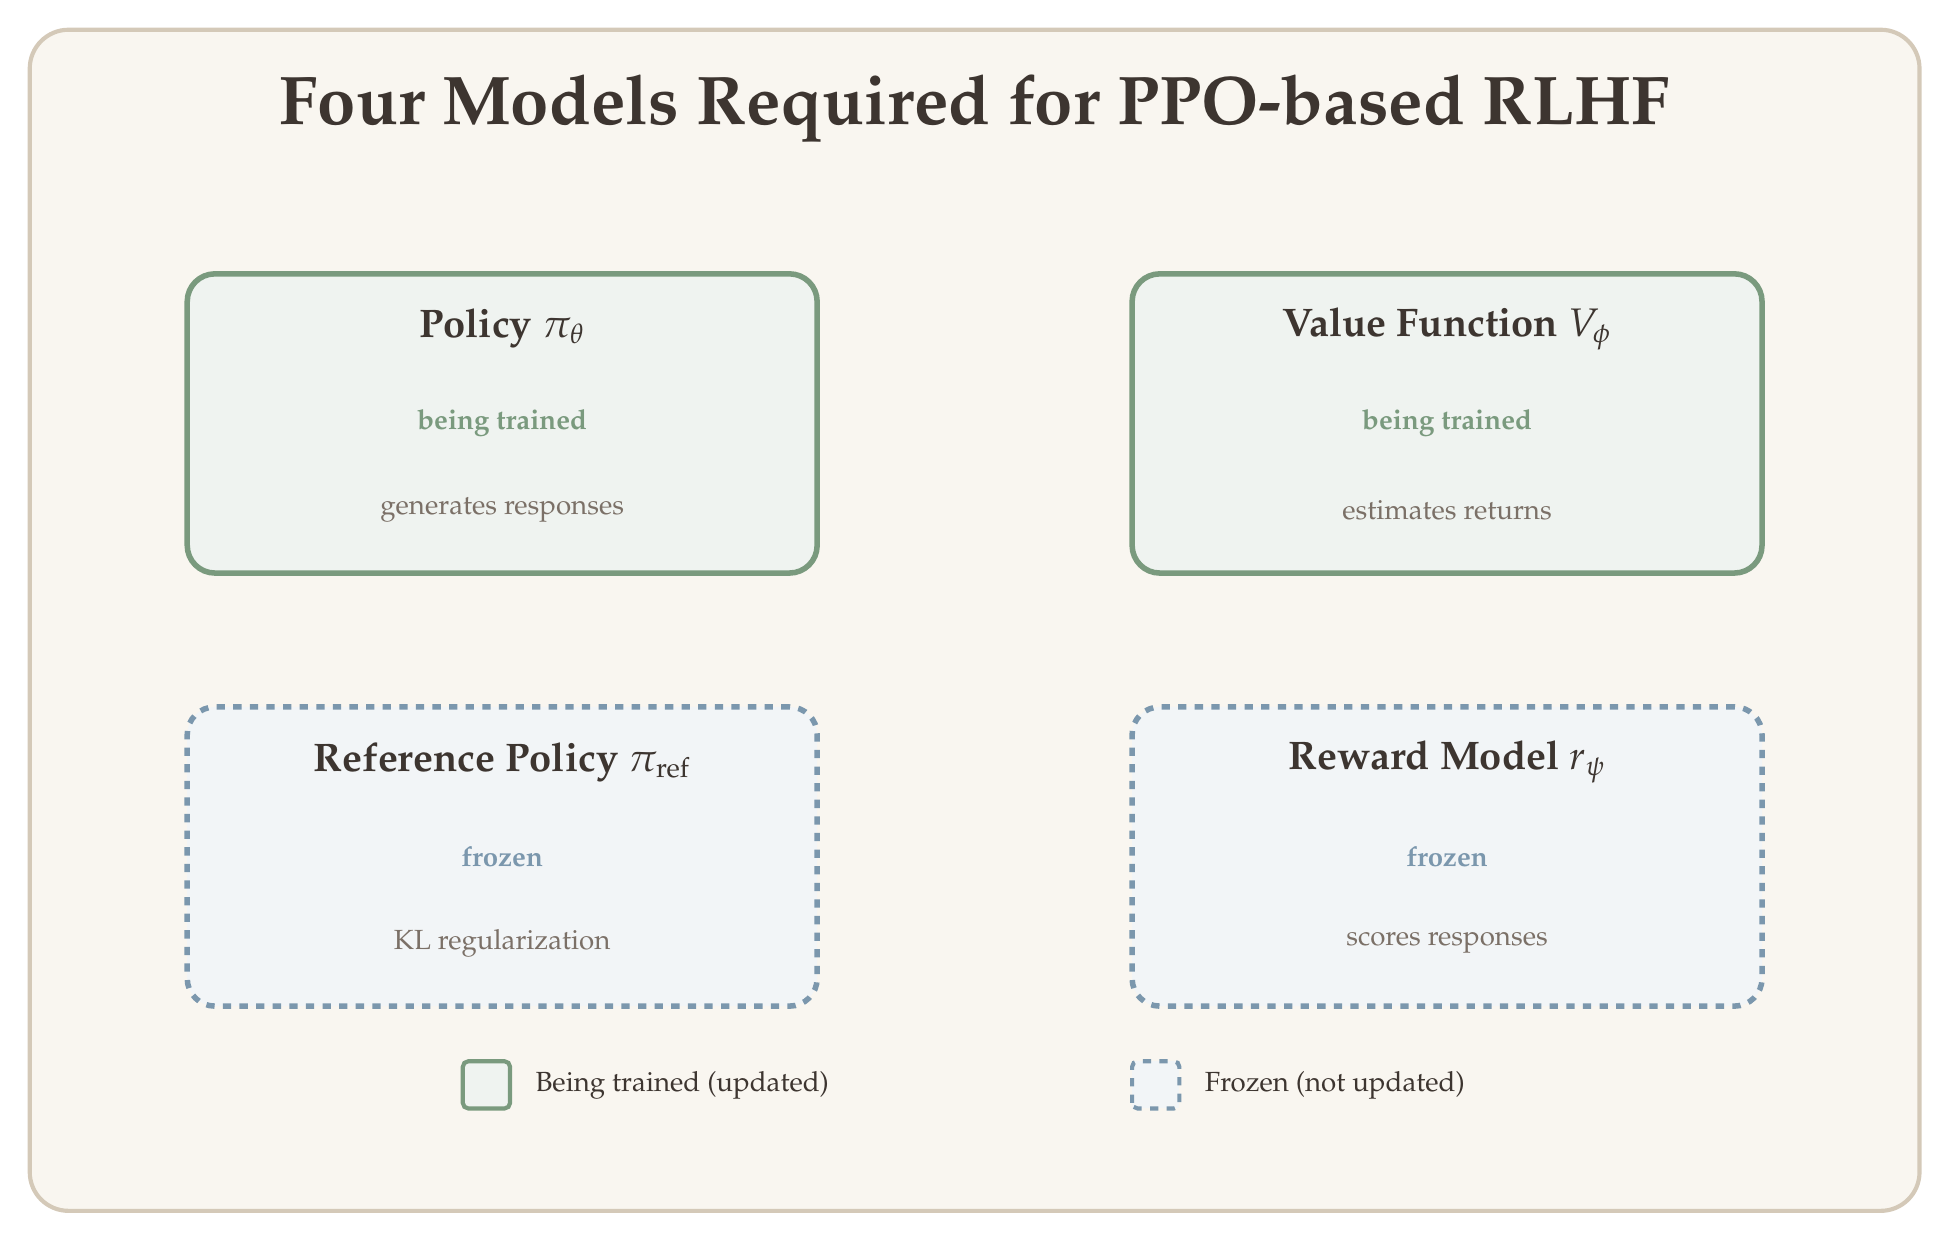
\begin{tikzpicture}[
  >={Stealth[length=3.5mm, width=2.5mm]},
  trainbox/.style={draw=sage, line width=2pt, fill=sage!12, rounded corners=10pt,
    minimum width=80mm, minimum height=38mm, font=\large, text=dkbrown,
    align=center, inner sep=10pt},
  frozenbox/.style={draw=stblue, line width=2pt, dashed, fill=stblue!10, rounded corners=10pt,
    minimum width=80mm, minimum height=38mm, font=\large, text=dkbrown,
    align=center, inner sep=10pt},
  statuslbl/.style={font=\normalsize\bfseries, rounded corners=3pt, inner sep=4pt},
]

% Background
\fill[cream, rounded corners=14pt] (-1.5,-7.5) rectangle (22.5,7.5);
\draw[border, rounded corners=14pt, line width=1.5pt] (-1.5,-7.5) rectangle (22.5,7.5);

% Title
\node[font=\Huge\bfseries, text=dkbrown] at (10.5,6.5)
  {Four Models Required for PPO-based RLHF};

% === Row labels ===
% Top row: being trained
% Bottom row: frozen

% === Top-left: Policy ===
\node[trainbox] (policy) at (4.5,2.5) {};
\node[font=\Large\bfseries, text=dkbrown] at (4.5,3.7) {Policy $\pi_\theta$};
\node[statuslbl, text=sage] at (4.5,2.5) {being trained};
\node[font=\normalsize, text=wmgray] at (4.5,1.4) {generates responses};

% === Top-right: Value Function ===
\node[trainbox] (value) at (16.5,2.5) {};
\node[font=\Large\bfseries, text=dkbrown] at (16.5,3.7) {Value Function $V_\phi$};
\node[statuslbl, text=sage] at (16.5,2.5) {being trained};
\node[font=\normalsize, text=wmgray] at (16.5,1.4) {estimates returns};

% === Bottom-left: Reference Policy ===
\node[frozenbox] (ref) at (4.5,-3) {};
\node[font=\Large\bfseries, text=dkbrown] at (4.5,-1.8) {Reference Policy $\pi_{\mathrm{ref}}$};
\node[statuslbl, text=stblue] at (4.5,-3) {frozen};
\node[font=\normalsize, text=wmgray] at (4.5,-4.1) {KL regularization};

% === Bottom-right: Reward Model ===
\node[frozenbox] (reward) at (16.5,-3) {};
\node[font=\Large\bfseries, text=dkbrown] at (16.5,-1.8) {Reward Model $r_\psi$};
\node[statuslbl, text=stblue] at (16.5,-3) {frozen};
\node[font=\normalsize, text=wmgray] at (16.5,-4.1) {scores responses};

% === Legend at bottom ===
% Green solid square
\fill[sage!12] (4.0,-6.2) rectangle (4.6,-5.6);
\draw[sage, line width=1.5pt, rounded corners=2pt] (4.0,-6.2) rectangle (4.6,-5.6);
\node[font=\normalsize, text=dkbrown, anchor=west] at (4.8,-5.9)
  {Being trained (updated)};

% Blue dashed square
\fill[stblue!10] (12.5,-6.2) rectangle (13.1,-5.6);
\draw[stblue, line width=1.5pt, dashed, rounded corners=2pt] (12.5,-6.2) rectangle (13.1,-5.6);
\node[font=\normalsize, text=dkbrown, anchor=west] at (13.3,-5.9)
  {Frozen (not updated)};

\end{tikzpicture}
\end{document}
